\chapter{Toolset for Analyzing Packet Flow in Interconnect}\label{sec:ii}

\section{Introduction}\label{sec:ii-introduction}

Inter-node communication performance of high-performance computing~(HPC)
clusters heavily affects the total performance of
communication-intensive applications. Communication-intensive
applications require low-latency and high-bandwidth communication
between compute nodes to fully exploit the computational power and
parallelism of the compute nodes. High performance networks that
provide such low-latency and high-bandwidth communication between
compute nodes of a cluster are often referred to as
\emph{interconnects}. Message Passing Interface
(MPI)~\autocite{MessagePassingInterfaceForum2015,Gropp2014} is a
commonly used inter-process communication library to describe
communication on HPC clusters.

In this dissertation, the interconnects are roughly classified into
\emph{static interconnects} and \emph{dynamic interconnects}. In the former
category, it is assumed that packet flow is statically controlled solely based
on its source and/or destination. A well-known exemplifier is
InfiniBand~\autocite{Buyya2009}, where forwarding tables held by switches are
populated with pre-computed forwarding rules in advance of the execution of
applications. In contrast, in the latter category, it is assumed that packet
flow is dynamically controlled to mitigate load imbalance and improve
utilization of the interconnect.

Nowadays, the majority of HPC clusters employ the former static interconnects
because of their technological maturity despite the potential cost advantage
dynamic interconnects could provide. The static interconnects are controlled
without taking the communication patterns of individual applications into
account. However, they are usually designed to be able to accommodate the
worst-case traffic demand to achieve good performance for a variety of
applications, each of which has a different communication pattern.
Interconnect designers have respected such criteria as full bisection
bandwidth and non-blocking networks.

The continuously growing demand for computing power from academia and
industry has inevitably forced HPC clusters to scale out more and more.
As a result of the growing number of compute nodes, interconnects
have been increasingly large-scale and complex. This technical trend is making
static and over-provisioned interconnects more cost-ineffective and
difficult to build.

Based on this background and these trends, this study explores the feasibility
and applicability of programming dynamic interconnect within
HPC~\autocite{Date2016}. In particular, \emph{SDN-enhanced
MPI}~\autocite{Takahashi2014,Dashdavaa2013}, a framework that incorporates
the dynamic network controllability of Software-Defined Networking
(SDN)~\autocite{sdn} into MPI, has been researched based on the idea that
dynamically optimizing the packet flow in the interconnect according to the
communication patterns of applications can increase the utilization of the
interconnect and then improve application performance. The goal of
SDN-enhanced MPI is to accelerate individual MPI collectives by dynamically
optimizing the packet flow in the interconnect. Several MPI collectives have
been successfully accelerated in the previous works so far. One of the core
challenges in the research on SDN-enhanced MPI lies in the design of an
algorithm to effectively control the packet flow in the interconnect for each
MPI collective called by the application.

More generally, an algorithm that takes the communication patterns of
applications as its input and then determines how to manage the packet flow
is essential towards realizing a dynamic and application-aware interconnect.
In order to develop a generic algorithm that achieves good performance on a
variety of applications and interconnects, the algorithm must be investigated
and evaluated by targeting different applications and interconnects. However,
utilizing actual clusters to analyze the performance characteristics of the
interconnect is restricted in the following three points. First, the execution
time of real-world HPC applications typically ranges from hours up to days,
sometimes even months. Second, large-scale deployments of dynamic
interconnects that allow execution of highly parallel applications have not
yet been seen because the research and development of dynamic interconnects
are still at their early stage. Third, network hardware such as switches may
not support measuring traffic in the interconnect with enough high frequency
and precision to obtain meaningful insights.

From the three restrictions mentioned above, an interconnect simulator that
allows users to conduct a systematic investigation of clusters with diverse
topologies and parameters is essentially demanded to accelerate the research
and development of application-aware dynamic interconnects that control packet
flow in response to the communication patterns of applications. A wide
spectrum of interconnect simulators have been developed with different focus
and purpose until today. However, existing simulators mostly focused on static
interconnects and few research has been done to simulate dynamic and
application-aware interconnects.

This chapter describes the design and implementation of PFAnalyzer, a
toolset for analyzing application-aware dynamic interconnects.
PFAnalyzer consists of two components: PFSim and PFProf. PFSim is an
interconnect simulator specialized for application-aware dynamic
interconnects. PFSim takes a set of communication patterns derived from
applications and a cluster configuration as its input and then simulates the
traffic on each link of the interconnect. PFProf is a custom profiler to
extract communication patterns from applications which are supplied to PFSim.

The contributions of this chapter are summarized as follows:

\begin{itemize}
\item
  A lightweight interconnect simulator for simulating dynamic and
  application-aware interconnects is proposed.
\item
  A custom profiler for extracting communication patterns from
  applications is presented.
\item
  Simulation results for NAS CG benchmark and MILC on a fat-tree
  interconnect are presented to demonstrate the practicality of of the
  proposed toolset.
\end{itemize}

The rest of this chapter is organized as follows.
Section~\ref{sec:ii-objective} examines the requirements of an
interconnect simulator for dynamic and application-aware interconnects.
Section~\ref{sec:ii-proposal} describes the design and implementation of
PFAnalyzer. Section~\ref{sec:ii-evaluation} evaluates the accuracy of the
simulated traffic. Furthermore, the NAS CG benchmark and MILC are taken as
example applications to demonstrate how PFAnalyzer can be used by researchers
to analyze the joint effect of node allocation, process placement and routing
on the distribution of traffic in the interconnect.
Section~\ref{sec:ii-related-work} reviews the related work.
Section~\ref{sec:ii-conclusion} concludes this chapter and outlines future
work.

\section{Research Objective}\label{sec:ii-objective}

% 大目標・シミュレーションを採用する理由
This chapter aims to realize a toolset for analyzing the packet flow in the
interconnect to facilitate the research and development of application-aware
dynamic interconnects. The packet flow generated in an interconnect highly
depends on parameters such as the communication pattern of application,
interconnect design and cluster configuration. When designing and implementing
an efficient application-aware dynamic interconnect, researchers need to
conduct a systematic analysis over many combinations of these parameters.
However, conducting such analysis on a physical cluster can be extremely time-
and resource-consuming. Therefore, this research takes the approach of
utilizing simulation to facilitate the analysis.

This research attempts to provide a toolset that performs a lightweight
simulation of the interconnect and predicts the packet flow generated in the
interconnect. The toolset should allow researchers to predict the packet flow
in the interconnect by supplying the communication pattern of real-world
application alongside with the interconnect design and cluster configuration.
The predicted packet flow can then be analyzed by researchers to gain an
insight on the interconnect while significantly saving the time and cost
compared to experiments on a physical cluster. Based on the discussion above,
the toolset should be able to satisfy the following requirements.

\begin{itemize}
\item
  \emph{Extraction of communication patterns from applications}:
  Communication patterns of real-world HPC applications should be fed
  into the simulator to reproduce the characteristics of communication
  generated by real-world applications. To simulate the packet flow in
  the interconnect when an application is being executed, the simulator
  needs to predict the volume of point-to-point communication exchanged
  between compute nodes. In the actual computing scene, the traffic
  among compute nodes is generated by the processes executed on the
  compute nodes. Thus, some means to analyze the traffic volume of
  point-to-point communication exchanged between the processes from
  applications is essential. In this chapter, applications that leverage
  MPI for inter-process communication are targeted.
\item
  \emph{Reproduction of process placement characteristic}:
  As described in Section~\ref{i:cluster-arch}, multiple jobs are running
  concurrently on a real-world cluster. Under such a cluster environment, the
  process placement characteristic of the job scheduler such as job
  scheduling, node selection and process placement algorithms heavily affect
  the distribution of packet flow generated in the interconnect. Since the
  job scheduler and its configuration largely varies across deployments,
  the process placement characteristic of the job scheduler needs to be
  reproduced.
\item
  \emph{Efficient prediction of packet flow in the interconnect}:
  The simulator should be designed to be lightweight and fast
  to carry out a large number of simulations with different parameters in
  a reasonable amount of time. If necessary, appropriate approximation
  should be introduced to improve simulation performance.
\end{itemize}

\section{Proposal}\label{sec:ii-proposal}

This research proposes \emph{PFAnalyzer}, a toolset for analyzing the
performance characteristics of application-aware dynamic interconnects.
PFAnalyzer is composed of \emph{PFProf}, a profiler to extract communication
patterns from applications, and \emph{PFSim}, a simulator capable of
simulating application-aware dynamic interconnects.

\subsection{Representation of a Communication Pattern}

In this dissertation, the communication pattern of an application is
represented using the traffic matrix of the application. The reason why this
research has adopt traffic matrix as representation of communication pattern
is explained below.

The traffic matrix of an application is defined as a matrix of which element
is equal to the traffic volume exchanged between two processes in the
application. Here, the volume of traffic between processes is approximated as
being constant during the execution of a job. In other words, The traffic
volume between a process pair is assumed to be the total bytes transferred
divided by the duration of the application.

This approximation is introduced to reduce the size of the communication
pattern as well as to simplify and to speed up the simulation. The idea behind
this approximation is based on the fact that many HPC applications
(\emph{e.g.} partial differential equation solvers) exhibit an iterative
nature. These applications spend most of their execution time inside a
repetitive loop and thus their communication patterns do not significantly
change over time. Therefore, omitting the temporal change of the communication
pattern and assuming the traffic volume between processes as being constant is
a good approximation. In the future, trace segmentation~\autocite{Alawneh2016}
techniques can be applied on the communication trace. This technique
segments a trace into multiple communication phases, which could then be
simulated individually to further improve the accuracy of simulation for
applications with significantly time-varying communication patterns.

\subsection{PFProf (MPI Profiler)}\label{sec:ii-pfprof}

% PFProfの概要
PFProf is a profiler that extracts the inter-process communication pattern
from MPI applications. The collected communication pattern is later fed into
PFSim to simulate the packet flow generated in the interconnect.

% プロファイリングを使う理由
To capture the inter-process communication of an MPI application, either
profiling or static analysis is commonly utilized. Profiling gives accurate
results but requires the user to run the application once. In contrast, static
analysis of the source code does not require the user to run the application.
However, the communication pattern obtained through the use of static analysis
is usually less accurate compared to the one obtained by profiling. This
research takes the profiling approach because an accurate communication
pattern is essential to obtain a simulation result with high fidelity.

% PMPIの問題点
Initially, existing MPI profilers and tracers such as
\mbox{Score-P}~\autocite{Knupfer2012}, Vampir~\autocite{Knupfer2008} and
TAU~\autocite{Shende2006} were considered for collecting the traffic matrices
from MPI applications. However, these tools can capture only a subset of the
communication pattern when profiling an application that uses MPI collectives.
The reason can be explained from the following technological aspect. Existing
MPI profilers replace the standard MPI functions provided by MPI libraries
with instrumented functions by utilizing the MPI Profiling Interface~(PMPI).
Although an advantage of this approach is that it works regardless of a
specific MPI implementation, this approach fails to capture the internal
information of the MPI library. Meanwhile, collective communication functions
are internally implemented as a combination of point-to-point communication in
MPI implementations. These underlying point-to-point communication functions
are hidden from PMPI-based profilers and excluded from the communication
patterns emitted by profilers.

% 集団通信を実現するアルゴリズムによっても変わる
Furthermore, the combination of point-to-point communication that composes a
collective communication is unknown until the execution of the application.
This is because MPI libraries usually implement multiple algorithms for each
MPI collective that are selected depending on the message size and number of
processes. For example, Open~MPI~\cite{Gabriel2004} implements three
algorithms to realize MPI\_Allgather: the recursive doubling algorithm, the
Bruck algorithm, and the ring algorithm~\cite{Rabenseifner2004}.
Figure~\ref{fig:allgather-algorithms} illustrates the underlying point-to-point
communication of MPI\_Allgather for each algorithm. It is evident that the
point-to-point communication of MPI\_Allgather is significantly different
depending on the algorithm being used.

\begin{figure}
    \centering
    \begin{subfigure}{\linewidth}
        \centering
        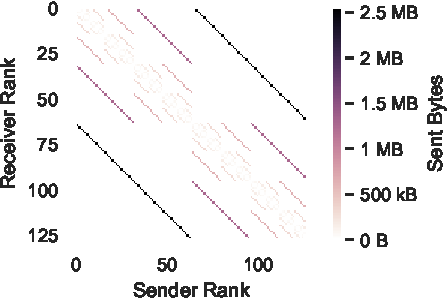
\includegraphics[width=.57\linewidth]{allgather_recursive_doubling}
        \caption{Recursive Doubling Algorithm}%
        \label{fig:allgather-recursive}
    \end{subfigure}
    \begin{subfigure}{\linewidth}
        \centering
        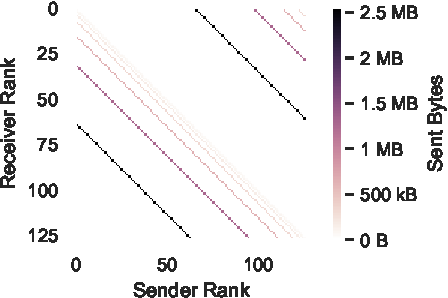
\includegraphics[width=.57\linewidth]{allgather_bruck}
        \caption{Bruck Algorithm}%
        \label{fig:allgather-bruck}
    \end{subfigure}
    \begin{subfigure}{\linewidth}
        \centering
        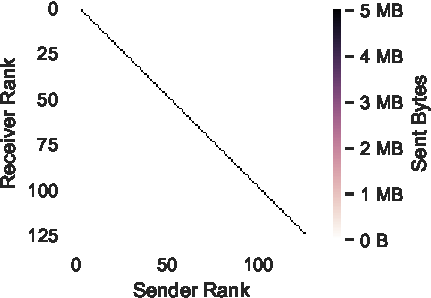
\includegraphics[width=.57\linewidth]{allgather_ring}
        \caption{Ring Algorithm}%
        \label{fig:allgather-ring}
    \end{subfigure}
    \caption{Underlying Point-to-Point Communication of MPI\_Allgather}%
    \label{fig:allgather-algorithms}
\end{figure}

% PERUSEを採用する理由
To accurately capture the underlying point-to-point communication of
collective communication, this research has taken the strategy of utilizing
the MPI Performance Examination and Revealing Unexposed State Extension
(PERUSE)~\autocite{Jones2006}. PERUSE was designed to provide the internal
information of an MPI implementation that was not exposed through PMPI to
applications and performance analysis tools. PERUSE delivers the internal
information of an MPI implementation to applications and performance analysis
tools through an event-driven API\@.

% アプリケーションの実行前の動作
Figure~\ref{fig:profiler-block} illustrates how PFProf, the MPI library and an
MPI application interact with one another. PFProf intercepts the function
calls from the application to several MPI functions using PMPI\@. MPI\_Init
and MPI\_Finalize are intercepted to perform initialization and finalization
when the application starts or exits (step~1 in
Fig.~\ref{fig:profiler-block}). In addition, PFProf intercepts MPI functions
that create or destroy communicators to maintain a mapping between global
ranks (rank number within \lstinline!MPI_COMM_WORLD!) and local ranks (rank
number within a communicator created by the user). This mapping is necessary
because PERUSE events are reported with local ranks, while profiling results
should be described with global ranks for the ease of analysis. During the
initialization, PFProf subscribes to two PERUSE events:
\lstinline!PERUSE_COMM_REQ_XFER_BEGIN! and
\lstinline!PERUSE_COMM_REQ_XFER_END! (step~2). These events are emitted each
time a transfer of a message begins and ends, respectively.

\begin{figure}
    \centering
    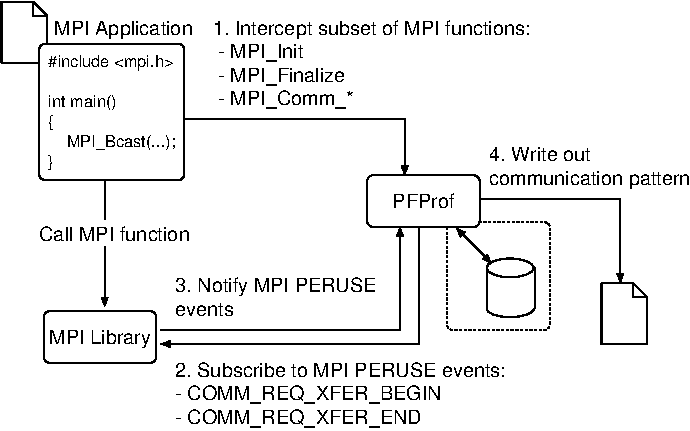
\includegraphics{tracer_block}
    \caption{Block Diagram of PFProf}%
    \label{fig:profiler-block}
\end{figure}

% アプリケーションの実行開始後の動作
After the application starts, PFProf receives PERUSE events from the MPI
library every time the application calls an MPI function that causes
inter-process communication (step~3). PERUSE extracts the sender, receiver and
transferred bytes from each PERUSE event and updates the traffic matrix
online. Once the application calls MPI\_Finalize, the communication pattern is
written out to disk as a JSON file (step~4).

% 共有ライブラリ
Finally, PFProf is designed to be provided in the form of a shared library so
that users do not need to modify the source code of their applications. Users
can either use the \lstinline!LD_PRELOAD! environment variable to load the
shared library at run-time or dynamically link the shared library with their
application at build-time.

\subsection{PFSim (Interconnect Simulator)}\label{sec:ii-pfsim}

% PFSimの概要
PFSim uses a set of communication patterns of applications and a cluster
configuration as its input and then simulates the packet flow generated
by the applications. The packet flow is aggregated per link to compute
the traffic load on each link. The simulated traffic load of links can
be summarized into statistics for quantitative analysis or visualized.
Using these outputs from PFSim, users can locate hot-spots and assess
load imbalance in the interconnect. These insights on the interconnect
can be useful for designing better algorithms for controlling the packet
flows in application-aware dynamic interconnects.

% シミュレーションの方式とモデル
Methodologies for simulating interconnects are roughly classified into
packet-level simulation~\cite{Hoefler2010} and flow-level
simulation~\cite{Schneider2009}. In the packet-level simulation, the behavior
of how each packet travels through the interconnect is precisely reproduced.
Therefore, the communication time of applications can be predicted accurately
in exchange for long execution time and large memory foot print. In contrast,
the flow-level simulation estimates the steady state behavior of the
interconnect and does not track individual packets. Thus, the packet flow in
the interconnect can be speedily estimated compared to the packet-level
simulation. As a trade-off, predicting the communication time of applications
using flow-level simulation is challenging. As described in
Section~\ref{sec:ii-objective}, this research aims at realizing a toolset for
efficiently predicting the packet flow in the interconnect under diverse
configurations. Therefore, PFSim is based on the flow-level simulation for
execution efficiency.

% シミュレータの構造
Figure~\ref{fig:pfsim-arch} shows the internal structure of PFSim. This
simulator is based on a discrete-event simulation model. Under this model, the
simulation is driven by events, each of which indicates a change in the
internal state of the simulator. Each event holds (1) type of the event, (2)
time when the event will occur, and (3) additional information. An event
queue is a priority queue that stores the events according to the time it will
occur. Event handlers are functions that are associated to a specific event
type and invoked when an event of the associated type occurs. The dispatcher
manages the event queue. It pops events from the event queue one by one and
calls the associated event handler for each event.

\begin{figure}
    \centering
    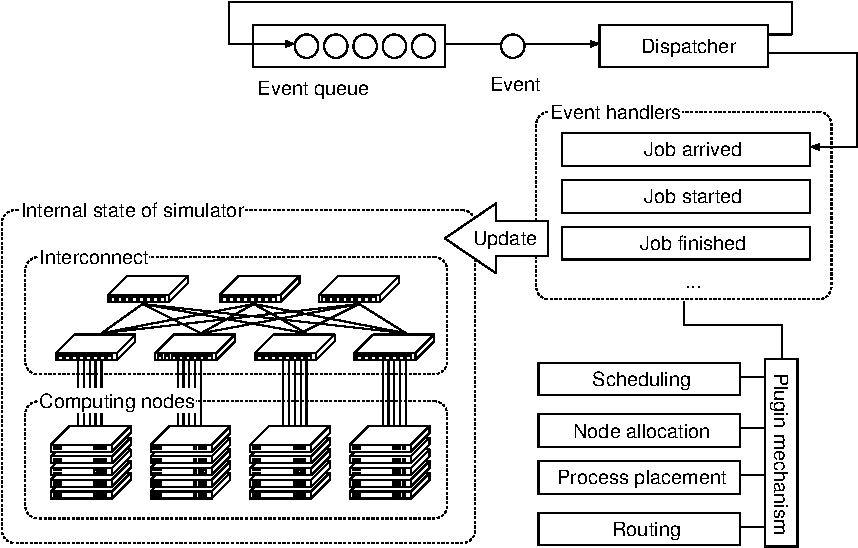
\includegraphics{pfsim-arch}
    \caption{Internal Structure of PFSim}%
    \label{fig:pfsim-arch}
\end{figure}

% ジョブ到着イベントハンドラ
In PFSim, three event types exist: job-arrived, job-started and job-finished.
The event handler for the job-arrived event first checks if the job queue is
empty and if there are enough compute nodes unallocated to run the job. If the
job is not runnable at the time, the job is enqueued to the job queue and the
event handler finishes. If the job is runnable, the event handler initiates
the job startup routine shown in Algorithm~\ref{alg:start-job}. First, a set
of available compute nodes are allocated to the job (line 1 in
Algorithm~\ref{alg:start-job}). Next, the placement of processes on the
allocated compute nodes is determined (line 2--3). Subsequently, each process
is associated to the compute node that accommodates it (line 4--5). Finally, a
job-started event is inserted into the event queue (line 6).

\begin{algorithm}
    \SetKwData{Job}{job}
    \SetKwData{Node}{node}
    \SetKwData{Nodes}{nodes}
    \SetKwData{Proc}{proc}
    \SetKwData{Procs}{procs}
    \SetKwData{Mapping}{mapping}
    \SetKwFunction{allocateNodes}{allocateNodes}
    \SetKwFunction{testNodes}{testNodes}
    \SetKwFunction{mapProcs}{mapProcs}

    \Nodes $\gets$ \allocateNodes{\Job}\;
    \Procs $\gets$ Set of processes composing \Job\;
    \Mapping $\gets$ \mapProcs{\Procs, \Nodes}\;
    \ForEach{(\Proc, \Node) $\in$ \Mapping}{%
        Associate \Proc with \Node\;
    }
    Insert job-started event to event queue\;

    \caption{Job start routine}%
    \label{alg:start-job}
\end{algorithm}

% ジョブ開始イベントハンドラ
Algorithm~\ref{alg:on-job-started} shows the overview of the event handler for
the job-started event. This event handler first obtains the traffic matrix of
the application that has started (line 1 in
Algorithm~\ref{alg:on-job-started}). Next, based on the traffic matrix, the
traffic load on each link in the interconnect is updated as follows: first,
compute nodes that accommodate the source and destination processes are
obtained (line 3--4). Subsequently, the path from the source compute node to
destination compute node is calculated (line 5--8). Lastly, the traffic load
on each link along the path is increased based on the amount of traffic
transferred between the source and destination processes (line 9--10). After
the traffic load is updated, the event handler inserts a job-finished event
into the job queue (line 11).

\begin{algorithm}
    \SetKwData{Job}{job}
    \SetKwData{SrcProc}{srcProc}
    \SetKwData{DstProc}{dstProc}
    \SetKwData{SrcNode}{src}
    \SetKwData{DstNode}{dst}
    \SetKwData{Link}{link}
    \SetKwData{Path}{path}
    \SetKwData{Traffic}{traffic}
    \SetKwData{TrafficMatrix}{tm}
    \SetKwFunction{route}{route}
    \SetKwFunction{selectJob}{selectJob}

    \TrafficMatrix $\gets$ Traffic matrix of \Job\;
    \ForEach{(\SrcProc, \DstProc, \Traffic) $\in$ \TrafficMatrix}{%
        \SrcNode $\gets$ Compute node that accommodates \SrcProc\;
        \DstNode $\gets$ Compute node that accommodates \DstProc\;
        \If{path between (\SrcNode, \DstNode) is already computed}{%
            \Path $\gets$ Cached path between (\SrcNode, \DstNode)\;
        }
        \Else{%
            \Path $\gets$ \route{\SrcNode, \DstNode, \Job}\;
        }
        \ForEach{\Link $\in$ \Path}{%
            Increase traffic load of \Link for \Traffic\;
        }
    }
    Insert job-finished event to event queue\;

    \caption{Event Handler for Job-started Event}%
    \label{alg:on-job-started}
\end{algorithm}

% ジョブ終了イベントハンドラ
The event handler for the job-finished event releases the compute nodes
allocated to the job. If there are one or more jobs in the job queue, one of
them is selected. If there are enough number of available compute nodes, the
job startup routine shown in Algorithm~\ref{alg:start-job} is invoked.

% シミュレーションシナリオファイルの概要
PFSim aims at predicting the packet flow in the interconnect generated by
applications under diverse cluster configurations. The configuration of the
simulation must be able to be edited by users. For the reason, the
configuration is described in a human-readable \emph{simulation scenario}
file. The simulation scenario file is designed to be described in a structured
serialization format called YAML\@. YAML has been adopted for its high
readability and editability compared to other alternatives such as JSON and
XML\@.

% シミュレーションシナリオファイルの詳細
Listing~\ref{lst:simulation-scenario} shows an example of a simulation
scenario file. In this simulation scenario file, the topology of the
interconnect (line 1 in Listing~\ref{lst:simulation-scenario}), output
directory for the simulation results (line 2), and a set of jobs to simulate
(line 16--21) are specified. Moreover, the algorithms that control the
execution and communication of jobs, which are shown in
Table~\ref{tbl:simulator-algorithm}, are also specified (line 3--15). Each
configuration value can be a list of parameters. The simulation is executed
multiple times, each time with a different combination of configuration values
until all combinations are completed. In
Listing~\ref{lst:simulation-scenario}, one scheduling algorithm (line 4--5),
two node allocation algorithms (line 6--8), two process placement algorithms
(line 9--11), and three routing algorithms (line 12--15) are specified. When
this scenario file is supplied to PFSim, 12 simulations are executed in total
in a combination manner.

\begin{lstlisting}[caption={Example of a Simulation Scenario},%
                   label={lst:simulation-scenario}, linewidth={\columnwidth},%
                   float={htbp}]
topology: topologies/milk.graphml
output: output/milk-cg-dmodk
algorithms:
  scheduler:
    - pfsim.scheduler.FCFSScheduler
  node_selector:
    - pfsim.node_selector.LinearNodeSelector
    - pfsim.node_selector.RandomNodeSelector
  process_mapper:
    - pfsim.process_mapper.LinearProcessMapper
    - pfsim.process_mapper.CyclicProcessMapper
  router:
    - pfsim.router.DmodKRouter
    - pfsim.router.GreedyRouter
    - pfsim.router.GreedyRouter2
jobs:
  - submit:
      distribution: pfsim.math.ExponentialDistribution
      params:
        lambd: 0.1
    trace: traces/cg-c-128.tar.gz
\end{lstlisting}

\begin{table}
    \centering
    \normalsize
    \caption{List of Configurable Algorithms}%
    \label{tbl:simulator-algorithm}
    \begin{tabularx}{\linewidth}{lX}
        \toprule
        Algorithm         & Description                                                 \\
        \midrule
        Job Scheduling    & Selects the job to execute from the job queue.
                            (\emph{e.g.} FCFS, Backfill)                                \\
        Node Selection    & Selects which compute nodes to assign for a job.
                            (\emph{e.g.} Linear, Random, Topology-aware algorithms)     \\
        Process Placement & Determines on which compute node to place a process.
                            (\emph{e.g.} Block, Cyclic, Application-aware algorithms)   \\
        Routing           & Computes a route between a pair of processes.
                            (\emph{e.g.} D-mod-K, S-mod-K, Random, Dynamic algorithms)  \\
        \bottomrule
    \end{tabularx}
\end{table}

Since PFSim accepts the topology of the interconnect as its input and outputs
the traffic load on each link of the interconnect, the file format for
representing the interconnect needs to be considered. The file format should
be designed for graphs since the interconnect can be considered as a graph. In
addition, the format should be supported by existing analysis and
visualization tools so that users can take advantage of these software assets.
Based on the requirements above, PFSim is designed to use
GraphML~\autocite{Brandes2013}, an XML-based markup language for graphs, as
its input and output format of the interconnect. Popular graph visualization
tools such as Cytoscape and Gephi can be used to view and edit GraphML files.
Users can use these tools to visually and intuitively locate bottleneck links
and load imbalance in the simulated interconnect.

\section{Evaluation}\label{sec:ii-evaluation}

The first experiment is conducted to verify if PFProf is able to capture
the underlying point-to-point communication behind collective communication.
Then, the accuracy of the simulation performed by PFSim is evaluated through
the comparison of the traffic estimated by PFSim with the traffic measured on
a cluster when actually running an application. Then, the performance of
point-to-point communication between two processes with and without PFProf are
compared to assess the overhead incurred by PFProf. Lastly, how PFAnalyzer can
be used by researchers to analyze the joint effect of node allocation, process
placement and routing on the distribution of traffic in the interconnect is
demonstrated.

\subsection{Comparison of PFProf and Conventional Profiler}%
\label{sec:ii-eval-pfprof}

This experiment verifies if PFProf is able to capture the underlying
point-to-point communication of collective communication. A simple
MPI application is profiled using TAU and PFProf. Subsequently, the extracted
communication patterns are compared. Listing~\ref{lst:pfprof-example} shows
the source code of the MPI application. This application first executes
MPI\_Allreduce, one of the commonly used collective communications. Then,
every process performs a point-to-point communication with its neighboring
process. This application is executed with 128 processes.

Figure~\ref{fig:tau-comm-matrix} shows the communication pattern obtained with
TAU\@. In this figure, the horizontal and vertical axis indicate the sender and
receiver rank, respectively. The point-to-point communication between the
neighbor processes is clearly visualized as a pattern along the diagonal.
However, the underlying point-to-point communication of MPI\_Allreduce was not
observed. On the other hand, Figure~\ref{fig:pfprof-comm-matrix} shows the
communication pattern obtained with PFProf. This communication pattern reveals
the MPI communication generated from MPI\_Allreduce in detail. The underlying
point-to-point communication is clearly detailed. These observations suggest
that PFProf is able to capture the underlying point-to-point communication of
collective communication.

\begin{lstlisting}[caption={MPI Application Used for Evaluation},
                   label=lst:pfprof-example, float, language=C]
#include <stdio.h>
#include <mpi.h>

#define BUF_SIZE    (1000)

int rank, size;
MPI_Request req;
char buf[BUF_SIZE] = {};
char buf2[BUF_SIZE] = {};

int main(int argc, char *argv[])
{
    MPI_Init(&argc, &argv);

    MPI_Comm_rank(MPI_COMM_WORLD, &rank);
    MPI_Comm_size(MPI_COMM_WORLD, &size);

    /* Collective communication */
    MPI_Allreduce(buf, buf2, BUF_SIZE, MPI_CHAR,
                  MPI_SUM, MPI_COMM_WORLD);
        \label{fig:allgather-ring}

    /* Point-to-point communication */
    MPI_Irecv(buf, BUF_SIZE, MPI_CHAR,
              (rank - 1) % size,
              0, MPI_COMM_WORLD, &req);
    MPI_Send(buf, BUF_SIZE, MPI_CHAR,
             (rank + 1) % size,
             0, MPI_COMM_WORLD);
    MPI_Wait(&req, MPI_STATUS_IGNORE);

    MPI_Finalize();
}
\end{lstlisting}

\begin{figure}
    \centering
    \begin{subfigure}{.49\linewidth}
        \centering
        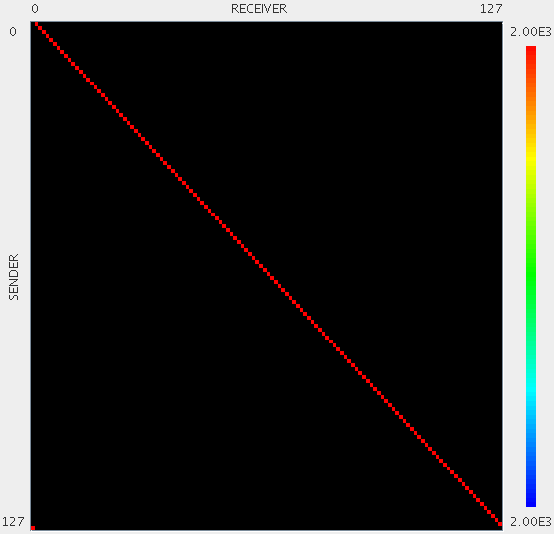
\includegraphics[width=.82\linewidth]{tau-comm-matrix}
        \caption{TAU}%
        \label{fig:tau-comm-matrix}
    \end{subfigure}
    \begin{subfigure}{.49\linewidth}
        \centering
        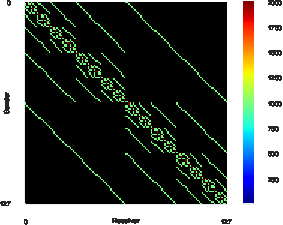
\includegraphics[width=.99\linewidth]{pfprof-comm-matrix}
        \caption{PFProf}%
        \label{fig:pfprof-comm-matrix}
    \end{subfigure}
    \caption{Extracted Communication Patterns}%
    \label{fig:profiler-comparison}
\end{figure}

\subsection{Accuracy of Traffic Estimated by PFSim}%
\label{sec:ii-eval-pfsim}

This experiment evaluates the accuracy of the simulation performed with PFSim.
The traffic estimated by PFSim and the traffic measured when running an
application on an actual cluster are compared.

The simulated cluster was modeled after a small-scale cluster installed at our
institution. The cluster is composed of 20 compute nodes, each equipped with
two quad-core Intel Xeon E5520 processors. Compute nodes are interconnected
with a two-tier fat-tree topology as illustrated in
Fig.~\ref{fig:cluster-config}. A single NEC ProgrammableFlow PF5240 switch is
logically divided into six switches that constitute the fat-tree topology.
The upper-layer two switches are referred to as spine1--spine2 and the
lower-layer four switches as leaf1--leaf4. The CG benchmark from the
NAS Parallel Benchmark Suite~\autocite{Bailey1991} was executed with 128
processes on 16 compute nodes. Since the CG benchmark only allows power-of-two
number of processes, some compute nodes could not be utilized.

\begin{figure}
    \centering
    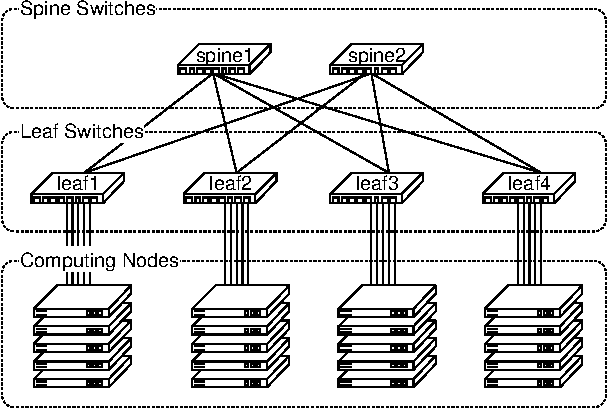
\includegraphics{pfsim-eval-cluster}
    \caption{Simulated Cluster with Fat-tree Interconnect}%
    \label{fig:cluster-config}
\end{figure}

Figure~\ref{fig:pfsim-accuracy} shows the comparison of simulated traffic
using PFSim and the measured traffic on the original cluster. The traffic on
each link between the spine switches and leaf switches were normalized by the
traffic on the link spine1$\rightarrow$leaf1 and shown in the plot. The plot
indicates the error of simulation result is small. The largest error was 1.9\%
and was observed on the link leaf4$\rightarrow$spine1. These results indicate
that the simulation result is sufficiently accurate to analyze performance of
dynamic interconnects.

\begin{figure}
    \centering
    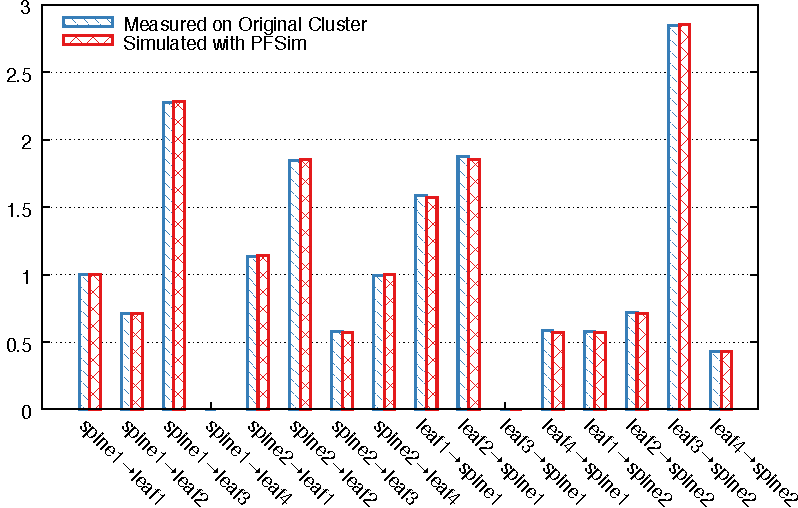
\includegraphics{pfsim-accuracy}
    \caption{Comparison of Simulated Traffic against Measured Traffic}%
    \label{fig:pfsim-accuracy}
\end{figure}

\subsection{Overhead Incurred by PFProf}

In this experiment, the performance of point-to-point communication
between two processes with and without PFProf were compared to inspect
the overhead incurred by the profiler. OSU Micro
Benchmark~\autocite{omb} was used to measure the throughput and latency
of point-to-point communication between two processes for varying
message sizes. The comparison of throughput and relative throughput are shown
in Fig.~\ref{fig:pfprof-bw-abs} and Fig.~\ref{fig:pfprof-bw-abs},
respectively. For messages larger than 1KB, the overhead was ignorable. For
messages smaller than 1KB, up to 30\% of overhead was incurred. Comparison of
latency and relative latency are shown shown in Fig.~\ref{fig:pfprof-lat-abs}
and Fig.~\ref{fig:pfprof-lat-rel}, respectively. These plots suggest that
there is almost no overhead for latency. These results indicate that PFProf is
able to extract the communication pattern from applications without
significantly hurting the performance of applications.

\begin{figure}
    \centering
    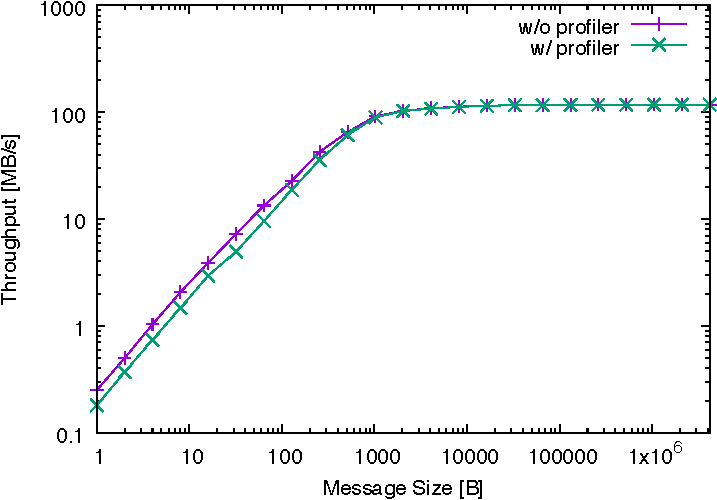
\includegraphics{pfprof_bandwidth_abs}
    \caption{Throughput of MPI\_Send/Recv Between Two Nodes}%
    \label{fig:pfprof-bw-abs}
\end{figure}

\begin{figure}
    \centering
    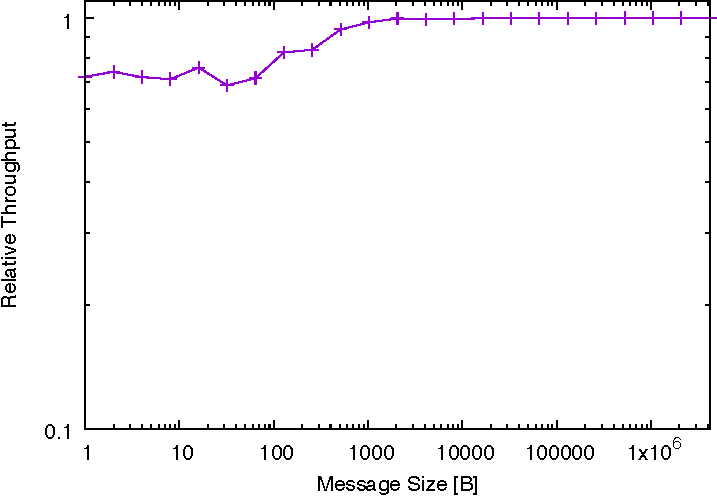
\includegraphics{pfprof_bandwidth_rel}
    \caption{Relative Throughput of MPI\_Send/Recv Between Two Nodes}%
    \label{fig:pfprof-bw-rel}
\end{figure}

\begin{figure}
    \centering
    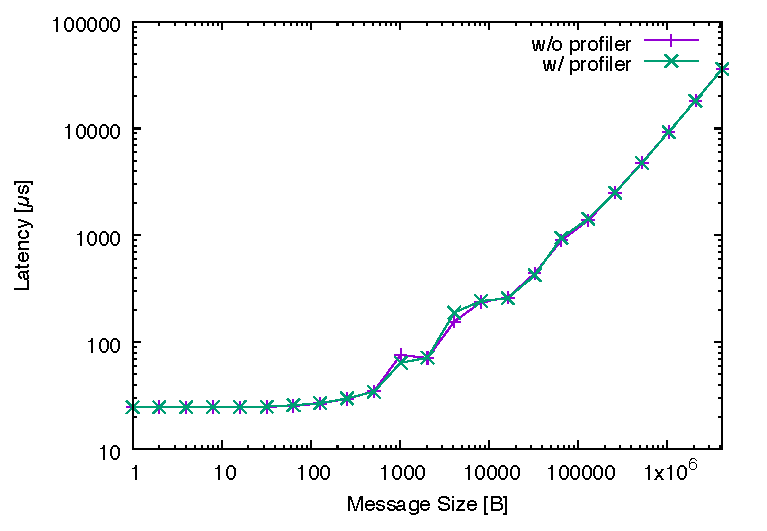
\includegraphics{pfprof_latency_abs}
    \caption{Throughput of MPI\_Send/Recv Between Two Nodes}%
    \label{fig:pfprof-lat-abs}
\end{figure}

\begin{figure}
    \centering
    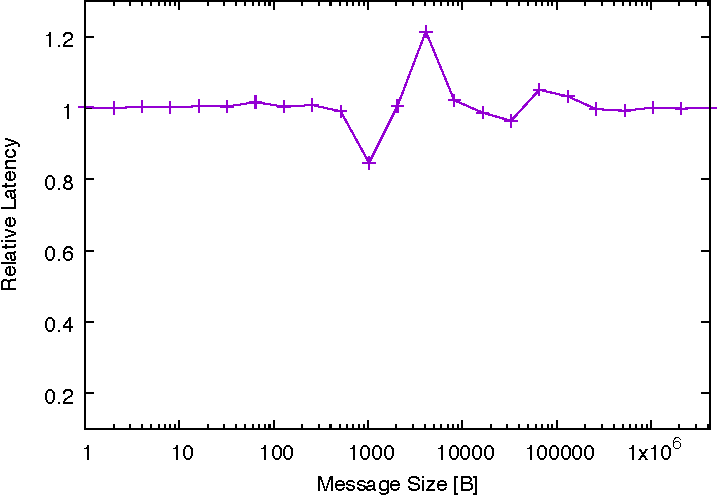
\includegraphics{pfprof_latency_rel}
    \caption{Relative Throughput of MPI\_Send/Recv Between Two Nodes}%
    \label{fig:pfprof-lat-rel}
\end{figure}

\subsection{Use Case of PFAnalyzer}\label{sec:ii-simulation-results}

This experiment shows how PFAnalyzer can be used by researchers to analyze the
joint effect of node allocation, process placement and routing on the
distribution of traffic in the interconnect. Communication-intensive MPI
applications were executed on the proposed simulator. The maximum traffic load
observed on links composing the interconnect was compared in both cases of
static interconnect control and dynamic interconnect control. The maximum
traffic load observed on the links was used as an indicator of the
communication performance of an application. In most cases, a hot spot link
can slow down the whole application, because every process needs to wait until
the slow communication crossing the hot spot link completes when collective
communication or synchronization is performed by an application. Therefore,
mitigating the traffic load on the hot spot link is considered to improve the
performance of the application.

Two applications were selected as representatives of communication-intensive
applications. The first one was the CG benchmark from the NAS Parallel
Benchmark Suite~\autocite{Bailey1991}. The CG benchmark estimates the largest
eigenvalue of a sparse matrix using the inverse power method. Internally it
uses the conjugate gradient method, which frequently appears in irregular mesh
applications. The second application (\lstinline!ks_imp_dyn!) was from MIMD
Lattice Computation (MILC)~\autocite{milc}, a collection of applications used
to study Quantum Chromodynamics (QCD). As for the input data, the data set
provided by NERSC as a part of the NERSC MILC benchmark was used. These two
applications were executed with 128 MPI processes. Thread parallelism was not
put in use (\emph{i.e.,} flat MPI model was adopted).

To analyze the effect of dynamic interconnect control, simulations were
carried out using static routing and dynamic routing control. Furthermore, in
order to investigate the impact of node selection and process placement to the
traffic load, the node selection algorithm and process placement algorithm
were also changed. As a result, exhaustive combinations of two node selection
algorithms, two process placement algorithms and two routing algorithms were
investigated with the scheduling algorithm fixed. Below are the descriptions
of the algorithms used in this experiment:

\begin{itemize}
\item
  Scheduling: A simple \emph{First-Come First-Served (FCFS)} scheduling
  without backfilling was adopted.
\item
  Node Selection: Either \emph{linear} or \emph{random} node selection
  was adopted. Linear node selection assumes that compute nodes are
  lined up in a one-dimensional array and minimizes the fragmentation of
  allocation. This is essentially the same as the default node selection
  policy of Slurm~\autocite{Yoo2003}. Random node selection, as the name
  indicates, randomly selects compute nodes. This algorithm simulates a
  situation where the allocation of compute nodes is highly fragmented.
\item
  Process Placement: Either \emph{block} or \emph{cyclic} process
  placement was adopted. Block process placement assigns rank \(i\) to
  the \(\lfloor i / c \rfloor\)-th compute node where \(c\) represents
  the number of cores per node. Cyclic process placement assigns rank
  \(i\) to the \((i \bmod n)\)-th compute node where \(n\) denotes the
  number of compute nodes.
\item
  Routing: Either \emph{D-mod-K} routing or a \emph{dynamic} routing was
  adopted. Destination-modulo-K (\mbox{D-mod-K}) routing is a
  popular static load balancing routing algorithm that distributes
  packet flow over multiple paths based on the destination address of
  the packet. The dynamic routing algorithm implemented here computes
  and allocates routes from the heaviest communicating process pair. A
  route is computed to minimize the traffic of the maximum-traffic link
  in the path.
\end{itemize}

Under this condition, the maximum traffic load observed on links through the
simulation were measured and compared.
Figure~\ref{fig:nas-cg-congestion} shows the simulation results in
the NAS CG benchmark. In this graph, the blue hatched bars represent the
results for \mbox{D-mod-K} routing while the red crosshatched bars represent
the results for dynamic routing. The vertical axis represents the simulated
maximum traffic load normalized by the maximum traffic load when linear node
selection, block process placement and \mbox{D-mod-K} routing were adopted.

What stands out in Fig.~\ref{fig:nas-cg-congestion} is that
dynamic routing consistently achieves lower traffic load compared to
static \mbox{D-mod-K} routing. The reduction of traffic load was the largest
when linear node selection and block process placement were adopted. Under
this combination of node selection and the process placement algorithm,
dynamic routing slashed the maximum traffic load by 50\% in comparison with
\mbox{D-mod-K} routing. Also, the graph reveals that cyclic process
placement always increased maximum traffic load compared to block process
placement because neighboring ranks were placed on different compute nodes
despite the locality of the communication pattern.

\begin{figure}
    \centering
    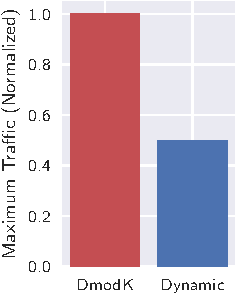
\includegraphics{nas_cg_congestion}
    \caption{Comparison of Maximum Traffic (NAS CG)}%
    \label{fig:nas-cg-congestion}
\end{figure}

\begin{figure}
    \centering
    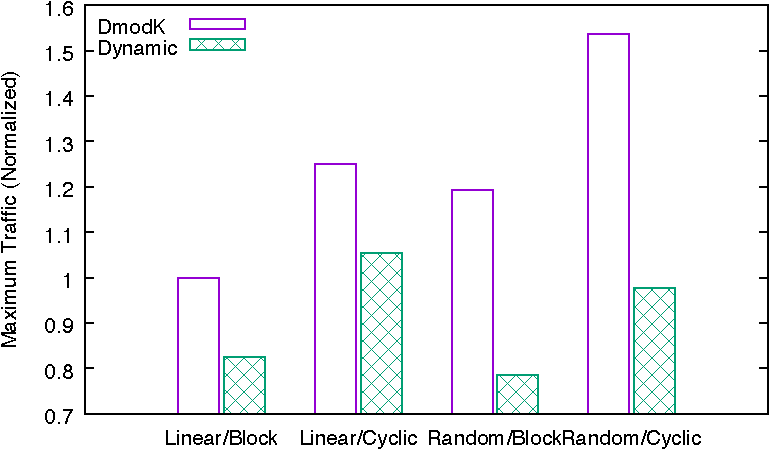
\includegraphics{nersc_milc_congestion}
    \caption{Comparison of Maximum Traffic (MILC)}%
    \label{fig:nersc-milc-congestion}
\end{figure}

Figure~\ref{fig:nersc-milc-congestion} shows the result in the case of
MILC\@. The graph reveals that dynamic routing outperforms \mbox{D-mod-K}
routing. In this case, the reduction of the link load was the largest when
random node selection and cyclic process placement was adopted. When using
linear node selection and block process placement, the reduction of the
maximum link load was 18\%. Compared to NAS CG benchmark, the effect of
dynamic routing was smaller.

To investigate the impact of traffic load on the application performance of an
actual environment, the configuration described in the previous
Section~\ref{sec:ii-simulation-results} was reproduced on a actual cluster and
then the execution time of each benchmark was measured. This cluster was
equipped with switches that support OpenFlow, which is a de facto standard
implementation of SDN\@. The routing algorithms were implemented based on
OpenFlow. In this experiment, linear node selection and block process
placement was adopted. The average execution time of 10 runs was compared when
using \mbox{D-mod-K} routing and dynamic routing. Figure~\ref{fig:cg-nersc-time}
shows the measured execution time for both benchmarks. The use of dynamic
routing reduced the execution time of NAS CG benchmark for 23\%. Meanwhile,
the execution time of MILC benchmark was reduced for 8\%, which was smaller
than the case of NAS CG benchmark. This matches with the simulation result
that predicted NAS CG benefits from larger reduction in maximum traffic load
by using dynamic routing compared to MILC\@.

These results suggest that application performance is actually improved
by alleviating the traffic load on the hot spot link. This suggestion
implies that researchers working on dynamic interconnects can take advantage
of the proposed toolset to simulate different packet flow controlling
algorithms and assess their performance improvement effect on real-world
applications by using indicators such as maximum traffic load.

\begin{figure}
    \centering
    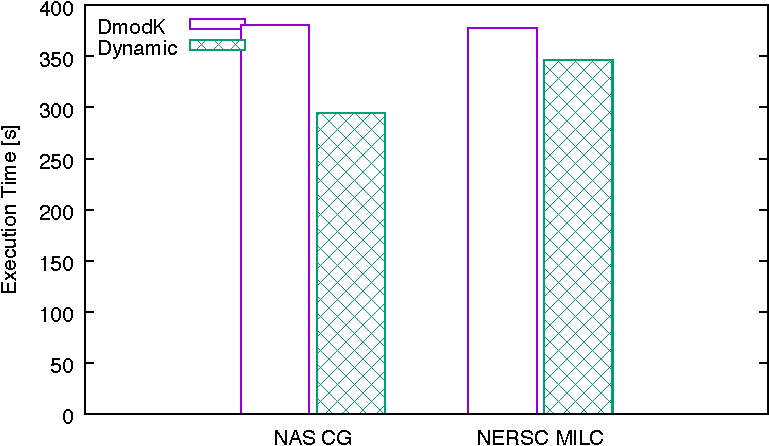
\includegraphics{pfsim_exec_time}
    \caption{Comparison of Execution Time on an Actual Cluster}%
    \label{fig:cg-nersc-time}
\end{figure}

\section{Related Work}\label{sec:ii-related-work}

Several interconnect simulators have been proposed in the past research.
PSINS~\autocite{Tikir2009} is a trace-driven simulator for HPC
applications. Traces obtained from applications are used to predict the
performance of applications on a variety of HPC clusters with different
configurations. LogGOPSim~\autocite{Hoefler2010} simulates the execution
of MPI applications based on the LogGOP network model. A limitation of
LogGOPSim is that the interconnect is assumed to have full bisection bandwidth
and thus congestion is not simulated. These two simulators can provide
accurate performance predictions owing to their per-message simulation
capability. However, the topology and the routing algorithm of interconnects
are abstracted in the network models of PSINS and LogGOPSim. Therefore, these
simulators cannot be used for predicting and comparing the performance of
different topologies or routing algorithms. In contrast, the simulator
proposed in this chapter allows users to compare the performance
characteristic of different topologies and routing algorithms.

ORCS~\autocite{Schneider2009} simulates the traffic load on each link in
the interconnect for a given topology, communication pattern and routing
algorithm in the same way as PFSim. The simulated traffic load of links can be
summarized into various performance metrics and used for further analysis. A
limitation of ORCS is that only pre-defined communication patterns can be used
as its input. Moreover, ORCS assumes static routing as in InfiniBand. On the
contrary, PFSim can handle dynamic routing algorithms that use communication
patterns of applications and interconnect usage to make routing decisions.

In~\autocite{Jo2015}, simulations are carried out to examine the
performance characteristics of an SDN-based multipath routing algorithm
for data center networks. A simulator was developed based on MiniSSF to
simulate the throughput and delay of a packet flow under diverse
settings. However, communication patterns are randomly generated and not
based on real-world applications. PFSim is designed to accept arbitrary
communication patterns obtained from real-world applications using our custom
profiler.

\(\mathit{INAM}^2\)~\autocite{Subramoni2016} is a comprehensive tool to
monitor and analyze network activities in an InfiniBand network. The
tight integration with the job scheduler and a co-designed MPI library
allows \(\mathit{INAM}^2\) to associate network activities with jobs and
MPI processes. For instance, it can identify hot spots in the
interconnect and inspect which node, job, and process is causing the
congestion. Although \(\mathit{INAM}^2\) is a useful tool for system
administrators to diagnose the performance issues of interconnects, it
is not suitable for studying diverse interconnects since it only
supports physical clusters.

\section{Conclusion}\label{sec:ii-conclusion}

This chapter described the design and implementation of PFAnalyzer, a
toolset for analyzing the performance characteristics of
application-aware dynamic interconnects. PFAnalyzer is composed of
PFProf, a profiler to extract communication patterns from applications,
and PFSim, a simulator capable of simulating application-aware dynamic
interconnects. PFSim takes a set of communication patterns of
applications and a cluster configuration as its input and then simulates
the traffic on each link of the interconnect. Evaluation conducted in this
dissertation verified that PFProf is able to capture the underlying
point-to-point communication of collective communication, which is essential
for understanding the communication characteristic of applications. Also, it
also indicated that the incurred overhead is small. Furthermore, the error of
traffic simulated with PFSim was 1.9\% at maximum, which is small enough to
analyze the performance characteristic of interconnects.

PFAnalyzer contributes to realizing a programmable interconnect control
adaptive to the communication pattern of application in two aspects. First,
PFProf allows researchers to accurately extract the inter-process
communication pattern from applications. The obtained communication pattern is
a crucial information for understanding the communication characteristic of
applications and adapting the interconnect control to the application. Second,
PFSim helps researchers to design and implement effective algorithms to
control the packet flow in the interconnect for mitigating imbalance in the
interconnect and achieving higher communication performance between compute
nodes.

Further work is necessary to investigate the performance characteristics of
dynamic interconnects on large-scale and highly parallel clusters. Moreover,
application-aware node selection and process placement algorithms are planned
to be implemented on PFSim. The impact of such application-aware algorithms on
the performance of dynamic interconnects should be evaluated.
